\section{Variable-Length Encoding Methods}
\label{sec:encoding}

\begin{figure}
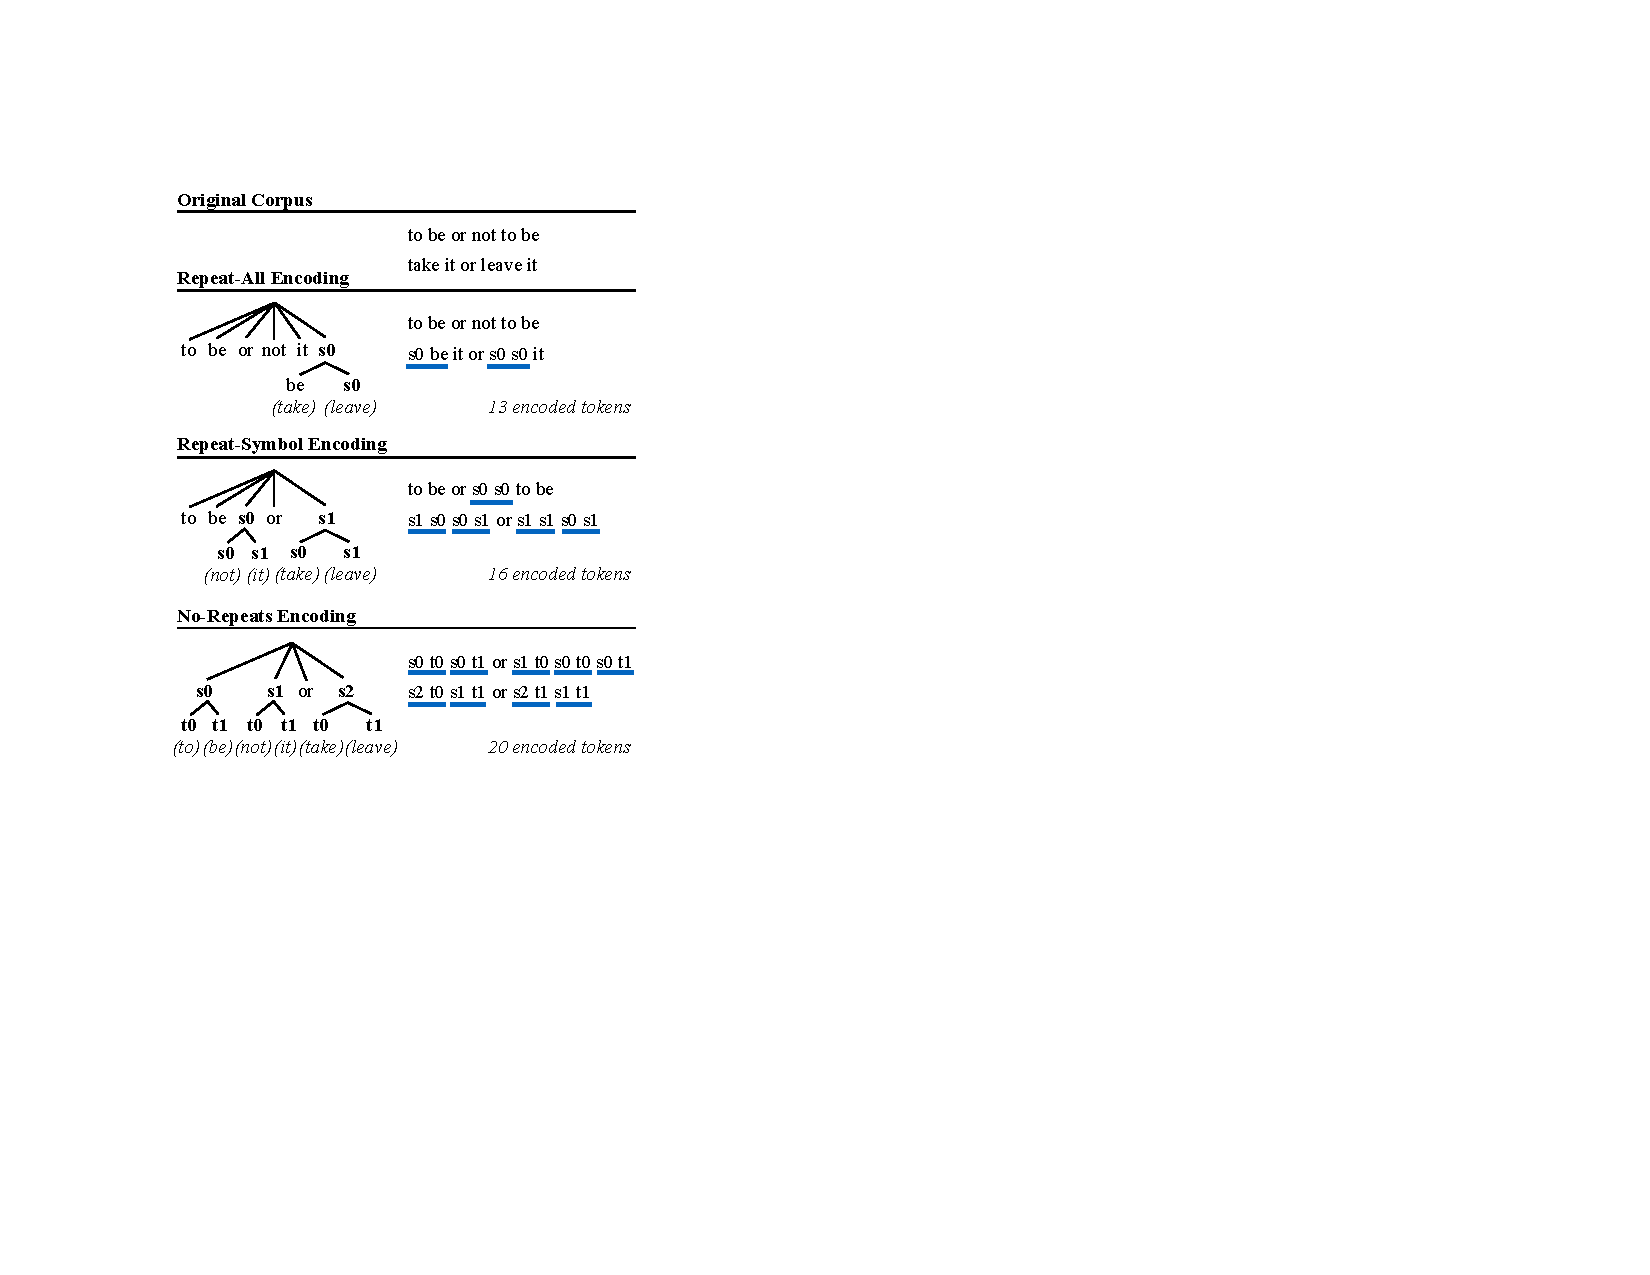
\includegraphics[width=3.1in]{examples}
\caption{Our three encoding schemes are applied to a two sentence toy corpus
for which each word type appears one or two times, and the total vocabulary
size $V$ is 7. An optimal encoding tree under each scheme is shown for an
encoded vocabulary size $W$ of 6. As stricter constraints are imposed on the
encoding, the encoded corpus length increases and the number of elements of $V$
that can be represented using a single symbol decreases. Two-symbol encodings
of rare words are underlined in blue.}
\label{fig:examples}
\end{figure}

We consider three different encoding schemes that are based on Huffman codes.
The encoding for a toy corpus under each scheme is depicted in
Figure~\ref{fig:examples}. While a Huffman code achieves the shortest possible
encoded length using a fixed vocabulary size $W$, symbols are often shared
between both common and rare words. Thus, a Huffman code may not be optimal for
the task of machine translation using a neural network model. The variants we
consider are designed to prevent specific forms of symbol sharing among
encodings.

\subsection{Encoding Schemes}

\noindent\textbf{Repeat-All.}
The first scheme is a standard Huffman code. In our experiments with
$V\approx2\cdot10^6$ and $W=3\cdot10^4$ and frequencies drawn from the Europarl
corpus, all words in $\mathcal{V}$ are encoded as either a single symbol or two
symbols of $\mathcal{W}$. We denote the single-symbol words (which have the
highest frequency) as ``common,'' and we call the other words ``rare.'' The
\emph{Repeat-All} encoding scheme has the most possible common words. In
Figure~\ref{fig:examples}, common words are represented as themselves. Rare
words are represented by two words, and the first is always a pseudo-word
symbol introduced into $\mathcal{W}$ of the form \textbf{sX} for an integer X.

\noindent\textbf{Repeat-Symbol.}
The emph{Repeat-Symbol} encoding scheme does not allow common-word symbols to
appear in the encoding of rare words. Instead, all rare words are encoded as
a two-symbol sequence of the form ``sX sX,'' where X are integers that may be
the same or different. This scheme decreases the number of common words in
order to encode all rare words using a restricted set of symbols. In this scheme, a common word in the encoded vocabulary always corresponds to a common word
in the original vocabulary.

\noindent\textbf{No-Repeats.}
Our final encoding scheme, \emph{No-Repeats}, uses a different vocabulary for
the first and second symbols in each rare word. That is, rare words are
represented as ``sX tX,'' where X are integers that may be the same or
different.  In this scheme, common words and rare words do not share symbols
and each symbol can be identified as common, the first of a rare pair, or the
second of a rare pair, without ever considering context.

\subsection{Symbol Counts}
To maximize performance, it is critical to set the number of common words (which
transform to themselves) as high as possible while satisfying the desired total vocabulary size,
counting all the newly introduced symbols. In this section, we algebraically derive
this optimal number of common words for each encoding scheme. We define the following:
\begin{description}
\item{$V$:} Size of the original vocabulary.
\item{$W$:} Size of the encoded vocabulary.
\item{$C$:} Number of common words.
\item{$S$:} Number of pseudo-words of the form \textbf{sX}.
\item{$T$:} Number of pseudo-words of the form \textbf{tX} (\emph{No-Repeats}).
\end{description}

We are interested in maximizing $C$ so that total encoding length is minimized.

\noindent\textbf{Repeat-All.}
We would like to encode the $V - C$ rare words, using only $W - C$ new symbols.
To do so, for each new symbol (non-terminal node in our encoding tree), we have
all $W$ symbols under it in that branch. Therefore, we maximize $C$ satisfying
the constraint that
$$V - C \leq (W - C) \cdot W$$

\noindent\textbf{Repeat-Symbol.}
Out of the $V - C$ rare words, we would like to pack them into a complete tree
so that they may be encoded using our remaining $W - C$ symbols. Therefore, we
maximize $C$ satisfying the constraint that
$$\sqrt{V - C} \leq W - C$$

\noindent\textbf{No-Repeats.}
Again, we desire to pack $V - C$ rare words into a complete tree where we may
use $V - C$ symbols. To maximize $C$, we let $S = T$. Because $S + T + C = W$,
we have that $2S + C = W$. Therefore, we maximize $C$ satisfying the constraint
that
$$\sqrt{V - C} \leq \frac{W - C}{2}$$
